%%%%%%%%%%%%%%%%%%%% author.tex %%%%%%%%%%%%%%%%%%%%%%%%%%%%%%%%%%%
%
% sample root file for your "contribution" to a contributed volume
%
% Use this file as a template for your own input.
%
%%%%%%%%%%%%%%%% Springer %%%%%%%%%%%%%%%%%%%%%%%%%%%%%%%%%%


% RECOMMENDED %%%%%%%%%%%%%%%%%%%%%%%%%%%%%%%%%%%%%%%%%%%%%%%%%%%
\documentclass[graybox]{svmult}

% choose options for [] as required from the list
% in the Reference Guide

\usepackage{mathptmx}       % selects Times Roman as basic font
\usepackage{helvet}         % selects Helvetica as sans-serif font
\usepackage{courier}        % selects Courier as typewriter font
\usepackage{type1cm}        % activate if the above 3 fonts are
                            % not available on your system
\usepackage{makeidx}         % allows index generation
\usepackage{graphicx}        % standard LaTeX graphics tool
                             % when including figure files
\usepackage{multicol}        % used for the two-column index
\usepackage[bottom]{footmisc}% places footnotes at page bottom
\usepackage{amsmath,amssymb,latexsym}

%% change footnote numbers to symbols
\renewcommand{\thefootnote}{\fnsymbol{footnote}}
%\newcommand{\bxi}{\ensuremath{\boldsymbol{\xi}}}
%\newcommand{\btheta}{\ensuremath{\boldsymbol{\theta}}}
% see the list of further useful packages
% in the Reference Guide

\makeindex             % used for the subject index
                       % please use the style svind.ist with
                       % your makeindex program

%%%%%%%%%%%%%%%%%%%%%%%%%%%%%%%%%%%%%%%%%%%%%%%%%%%%%%%%%%%%%%%%%%%%%%%%%%%%%%%%%%%%%%%%%

\begin{document}

\title*{Bayesian Inference of Stochastic Pursuit Models from Basketball Tracking Data}
\titlerunning{Stochastic Pursuit and Basketball}
% Use \titlerunning{Short Title} for an abbreviated version of
% your contribution title if the original one is too long
\author{Harish S. Bhat, R. W. M. A. Madushani, and Shagun Rawat}

% Use \authorrunning{Short Title} for an abbreviated version of
% your contribution title if the original one is too long
\institute{Harish S. Bhat \at University of California Merced, 5200 N. Lake Rd., Merced, CA, USA \\ \email{hbhat@ucmerced.edu}
\and R. W. M. A. Madushani \at University of California Merced, 5200 N. Lake Rd., Merced, CA, USA \\ \email{rmadushani@ucmerced.edu}
\and Shagun Rawat \at University of California Merced, 5200 N. Lake Rd., Merced, CA, USA \\ \email{srawat2@ucmerced.edu}
}

%
% Use the package "url.sty" to avoid
% problems with special characters
% used in your e-mail or web address
%
\maketitle

\abstract*{We develop a Metropolis algorithm to perform Bayesian inference for models given by coupled stochastic differential equations. A key challenge in developing practical algorithms is the computation of the likelihood. We address this problem through the use of a fast method to track the probability density function of the stochastic differential equation.  The method applies quadrature to the Chapman-Kolmogorov equation associated with a temporal discretization of the stochastic differential equation.  The inference method can be adapted to scenarios in which we have multiple observations at one time, multiple time series, or observations with large and/or irregular temporal spacing.  Computational tests show that the resulting Metropolis algorithm is capable of efficient inference for an electrical oscillator model.}

\section{Introduction}
\label{sec:1}

In 2010, the National Basketball Association (NBA) began to install a
camera system to track the positions of the players and the ball as a
function of time.  For the ball and for each of the $10$ players on
the court, the system records an $(x,y)$ position $25$ times per
second.  Ultimately, this wealth of data should enable us to answer a 
number of questions regarding basketball strategy that would have
seemed intractable just a few years ago.  To bring this vision to
reality, we must develop new algorithms that can efficiently use the
data for inference of appropriate models.

In this work, we focus on so-called ``fast break'' situations where an
offensive player races towards the basket in an attempt to score before the
defensive team has time to set up their defense.  In many such situations,
it is relatively easy to identify from the data a runner and a
chaser.  This motivates the following question that is central to the
present paper: using the NBA's spatial tracking data, how can we infer
a stochastic model for the chaser's pursuit of the runner?

To answer this question, we first formulate a stochastic version of
the classical pursuit model.  Our model consists of a set of coupled,
nonlinear stochastic differential equations with time-dependent
coefficients.  To perform Bayesian inference for this stochastic
model, we develop a Markov Chain Monte Carlo (MCMC) algorithm.  The
MCMC algorithm is derived using a Metropolis scheme; our innovation is
to evaluate the log likelihood efficiently using a novel, deterministic
method called density tracking by quadrature (DTQ).  The DTQ method
applies quadrature to the Chapman-Kolmogorov equation associated with
a time-discretization of the original stochastic differential equation
(SDE) \cite{BhatMadu2016}. For the case of scalar SDE, the DTQ
method's density function converges to the true density of the SDE at
a rate that is linear in the time step.

Note that the MCMC algorithm developed here can be applied for
Bayesian inference of a class of two-dimensional SDE, not just the pursuit model
considered here.  Note that inference of SDE models is a 
challenging problem, due to the fact that a closed-form likelihood
function is generally unavailable \cite{sorensen2004parametric,
  iacus2009simulation, fuchs2013inference}. Most existing parametric
inference methods for discretely observed SDE require
inter-observation times to be small.  As a way to facilitate
approximation of the transition density for parametric inference for
large inter-observation times, Bayesian methods are used to simulate
missing values of the observations to form a high-frequency data
set. In situations where the likelihood function is either
analytically unavailable or computationally prohibitive to evaluate,
Bayesian inference of SDE makes use of likelihood-free methods such as
Approximate Bayesian Computation \cite{Picchini2014}, variational
methods \cite{Archambeau2007a, Vrettas2015}, and/or Gaussian processes
\cite{Archambeau2007, Ruttor2013}.  In ongoing and future work, we
will conduct a careful comparison of our method against these other
methods.  For the purposes of the present paper, we are more
interested in establishing the appropriateness of a stochastic pursuit
model for basketball fast breaks.

%SDE have application in areas epidemiology, mechanics, genetics, population biology, systems biology, molecular dynamics, geostatistics,social sciences, economics and finance. (include why parameter estimation is important, existing methods and the challenge of computation of the likelihood)

%In our work we have developed a Markov Chain Monte Carlo Method (MCMC) algorithm for Bayesian inference of parameters in SDE.    The method we have developed is applicable to the case where inter-observation times are large and/or irregular.  In this paper, we present a Metropolis algorithm for Bayesian inference of unknown parameters of a 2-D SDE.

\section{Derivation of the Model and Inference Method}
\label{sec:2}
Let the \emph{runner} be the player (on offense) who has the ball and
is running toward the basket.  Let the \emph{chaser} be the player (on
defense) who is trying to prevent the runner from scoring.   Let the
current spatial coordinates of the runner and chaser be, respectively,
$(x^{r}(t), y^{r}(t))$ and $(x^{c}(t), y^{c}(t))$.

\begin{figure}[tb]
\centering
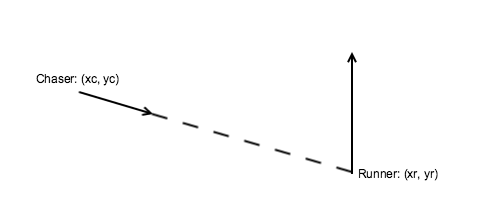
\includegraphics[width=0.8\textwidth]{pursuit.png}
\caption{Diagram illustrating motion of runner and chaser.  At any
  instant of time, the chaser's velocity vector points toward the
  runner's current position.}
\label{fig:pursuitdiagram}
\end{figure}

Consider the diagram in Figure \ref{fig:pursuitdiagram}.  Since the
chaser is moving towards the runner, the velocity vector of the chaser
points toward the runner's current position.  Let $\vec{\phi} = (x^{r}
- x^{c}, y^{r} - y^{c})$. Then the unit vector that points toward the
runner from the chaser is $\phi / \| \phi \|$.  The velocity of the chaser, $(\dot{x}^c, \dot{y}^c)$, can thus be given as
\begin{equation}
\label{eqn:pursuitODE}
(\dot{x}^c, \dot{y}^c) = \gamma(t) \frac{\phi}{\| \phi \|},
\end{equation}
where $\gamma(t) = \| (\dot{x}^c,\dot{y}^c) \|$, the instantaneous
speed of the chaser.  Note that (\ref{eqn:pursuitODE}) is a coupled
system of nonlinear ordinary differential equations known as the
pursuit model---classically, one assumes that
$\gamma(t)$ and $(x^{r}(t),y^{r}(t))$ are given, in which case one
typically solves an initial-value problem for $(x^{c}(t),y^{c}(t))$.
To generalize the classical model to the real data context considered
here, we multiply both sides of (\ref{eqn:pursuitODE}) by $\mathrm{d}t$ and
then add noise to each component:
\begin{equation}
\label{eqn:pursuitSDE}
\mathrm{d}(x^{c}, y^{c}) = \gamma(t) \frac{\vec{\phi}}{ \|
                           \vec{\phi} \| } \mathrm{d}t + (\nu_1
                         \mathrm{d}W^1_t, \nu_2 \mathrm{d}W^2_t)
\end{equation}
Here $W_{1,t}$ and $W_{2,t}$ denote two independent Wiener processes
with $W_{1,0} = W_{2,0} = 0$ almost surely.  We refer to this model as
the stochastic pursuit model.

Given time-discrete observations of
$(x^{c},y^{c})$ and $(x^{r},y^{r})$, how do we infer $\gamma(t)$
together with $\nu_1$ and $\nu_2$?  Our first step is to consider
(\ref{eqn:pursuitSDE}) as a particular example of a more general class of systems:
\begin{subequations}
\label{eqn:sde}
\begin{align}
\mathrm{d}X_{1,t} &= f_1(t, \mathbf{X}_t, \theta)\mathrm{d}t + g_1(t, \mathbf{X}_t, \theta) \mathrm{d}W_{1,t} \\
\mathrm{d}X_{2,t} &= f_2(t, \mathbf{X}_t, \theta)\mathrm{d}t + g_2(t, \mathbf{X}_t, \theta) \mathrm{d}W_{2,t}.
\end{align}
\end{subequations}
Here $\mathbf{X}_t = (X_{1,t}, X_{2,t})$ is a two-dimensional
stochastic process. For $j=1, 2$, we refer to $f_j$ and $g_j$ as,
respectively, drift and diffusion functions.  Both
drift and diffusion functions may depend on a parameter vector
$\theta \in \mathbb{R}^{N}$.

For the stochastic pursuit model (\ref{eqn:pursuitSDE}), we take
$\mathbf{X}_t = (x^{c}(t), y^{c}(t))$.  We treat $\gamma(t)$ as
piecewise constant.  Each constant value of $\gamma(t)$ is one
component of the parameter vector $\theta$; the final two
values of this vector are $\nu_1$ and $\nu_2$.  Finally, if we treat
$(x^{r}(t), y^{r}(t))$ as given, then we can identify the time-dependent drift
functions $f_1$ and $f_2$ as the two components of $ \gamma(t) \phi /
\| \phi \|$. 

Our goal is to infer $\theta$ from direct, discrete-time observations of $\mathbf{X}_t$.  Suppose that at a sequence of times $0 = t_0 < t_1 < \cdots < t_M = T$, we have observations $\mathbf{x} := \{({x}_{1,m},{x}_{2,m})\}_{m=0}^M$.  Here $\mathbf{x}_m = ({x}_{1,m},{x}_{2,m})$ is a sample of $\mathbf{X}_{t_m}$.  In this paper, we will assume equispaced temporal observations, i.e., $t_m = m \Delta t$ for fixed step size $\Delta t > 0$.  We make this assumption purely for notational simplicity; the method we describe can be easily adapted for nonequispaced temporal observations.  We refer to $\Delta t$ as the time step of the data.

The posterior density of the parameter vector given the observations is
$p(\theta \, | \, \mathbf{x})  \propto p( \mathbf{x} \, | \, \theta)  p(\theta)$,
where $p( \mathbf{x} \, | \, \theta)$ is the likelihood and $p(\theta)$ is the prior.  We discretize the SDE (\ref{eqn:sde}) in time using the Euler-Maruyama scheme:
\begin{subequations}
\label{eqn:discretesde}
\begin{align}
X_1^{n+1} &= X_1^{n} + f_1(t_n, X_1^n, X_2^n, \theta)h + g_1(t_n, X_1^n, X_2^n,  \theta) \sqrt{h} Z_1^{n+1} \\
X_2^{n+1} &= X_2^{n} + f_2(t_n, X_1^n, X_2^n,\theta)h + g_2(t_n, X_1^n, X_2^n,\theta) \sqrt{h} Z_2^{n+1}.
\end{align}
\end{subequations}

Here $h > 0$ is a fixed time step, the time step of our numerical method.  We shall choose $h$ to be a fraction of $\Delta t$, i.e., $F h = \Delta t$ for integer $F \geq 2$.  The random variables $X_i^n$ for $i=1,2$ are approximations of $X_{i,n h}$.  The $Z_i^n$ are independent and identically distributed random variables, normally distributed with mean $0$ and variance $1$, i.e., $Z_i^n \sim \mathcal{N}(0,1)$.

Let $\widetilde{p}(\mathbf{x} \, | \, \theta)$ denote the likelihood under the discrete-time model (\ref{eqn:discretesde}), an approximation to the true likelihood $p(\mathbf{x} \, | \, \theta)$.  Note that (\ref{eqn:discretesde}) describes a discrete-time Markov chain.  By the Markov property, the likelihood $\widetilde{p}(\mathbf{x} \, | \, \theta)$ factors and we can write:
\begin{equation}
\label{eqn:markovfactor}
p(\mathbf{x} \, | \, \theta) \approx \widetilde{p}(\mathbf{x} \, | \, \theta) = \prod_{m=0}^{M-1} \widetilde{p}(\mathbf{x}_{m+1} \, | \, \mathbf{x}_m, \theta).
\end{equation}
The term $\widetilde{p}(\mathbf{x}_{m+1} \, | \, \mathbf{x}_m, \theta)$ is the transition density for (\ref{eqn:discretesde}), from state $\mathbf{x}_m$ at time $t_m$ to state $\mathbf{x}_{m+1}$ at time $t_{m+1}$.  This suggests a numerical method for computing this density, which we explore in the next subsection.
 
\subsection{Density Tracking by Quadrature (DTQ)}
\label{subsec:2-1}
Equation (\ref{eqn:discretesde}) describes a Markov chain over a continuous state space.  If we let $\widetilde{p}^n(x_1,x_2 \, | \, \theta)$ denote the joint probability density function of $X_1^n$ and $X_2^n$ given $\theta$, then the Chapman-Kolmogorov equation associated with (\ref{eqn:discretesde})  is
\begin{equation}
\label{eqn:chapman}
\widetilde{p}^{n+1}(x_1,x_2 \, | \, \theta) = \int_{y_1,y_2 \in \mathbb{R}^2} K(x_1,x_2,y_1,y_2,t_n; \theta) \widetilde{p}^n(y_1,y_2 \, | \, \theta) \, dy,
\end{equation}
where
\begin{align}
&K(x_1,x_2,y_1,y_2,t_n; \theta) = \widetilde{p}^{{n+1} | {n}}(x_1,x_2 | y_1,y_2,\theta) \nonumber\\
&= (2 \pi \sigma_1^2)^{-1/2} \exp \left[ -(x_1 - \mu_1)^2/(2 \sigma_1^2) \right] (2 \pi \sigma_2^2)^{-1/2} \exp \left[ -(x_2 - \mu_2)^2/(2 \sigma_2^2) \right]\nonumber.
\end{align}
Here $\mu_1 = y_1 + f_1(t_n,y_1,y_2; \theta) h,  \mu_2 = y_2 + f_2(t_n,y_1,y_2; \theta) h,  \sigma_1^2 = g_1^2(t_n,y_1,y_2; \theta) h$ and  $\sigma_2^2 = g_2^2(t_n,y_1,y_2; \theta) h$. That is, $K(x_1,x_2,y_1,y_2,t_n; \theta)$ is the conditional density of $X_1^{n+1}$ and $X_2^{n+1}$ given $X_1^n = y_1$, $X_2^n = y_2$ and $\theta = \theta$, evaluated at the point $(x_1,x_2)$.  The fact that the conditional density is a product of normal distributions with means $\mu_1, \mu_2$ and variances $\sigma_1^2, \sigma_2^2$ can be shown using (\ref{eqn:discretesde}) together with the fact that $X_1^{n+1}$ and $X_2^{n+1}$ are conditionally independent given $X_1^n$ and $X_2^n$. This conditional independence is a direct consequence of having two independent random variables $Z_1^n$ and $Z_2^n$ in (\ref{eqn:discretesde}).

The crux of the DTQ method is to apply quadrature to (\ref{eqn:chapman}) to evolve an initial density forward in time.  Consider a spatial grid with fixed spacing $k > 0$ and grid points $x_1^i = ik$, $x_2^j = jk$, $y_1^{i'} = i'k$, and $y_2^{j'} = j'k$.  Then we apply the trapezoidal rule in both the $y_1$ and $y_2$ variables to obtain:
\begin{equation}
\hat{p}^{n+1}(x_1^i, x_2^j ;\theta) = k^2 \sum\limits_{i' = -\infty}^{\infty} \sum\limits_{j' = -\infty}^{\infty} K(x_1^i, x_2^j, y_i^{i'}, y_2^{j'},t_n; \theta)  \hat{p}^n(y_1^{i'}, y_2^{j'}; \theta)
\end{equation}
It is unnecessary to sum over all of $\mathbb{Z}^2$.  We know that a two-dimensional Gaussian decays to zero far from its mean.  Since the mean $(\mu_1,\mu_2)$ is approximately $(y_1,y_2)$, we sum only from $y_1 = x_1 - \zeta k$ to $y_1 = x_1 + \zeta k$ and similarly for $y_2$:
\begin{equation}
\label{eqn:phatalg}
\hat{p}^{n+1}(x_1^i, x_2^j;\theta ) = k^2 \sum\limits_{i' = i - \zeta}^{i+ \zeta} \sum\limits_{j' = j-\zeta}^{j+\zeta} K(x_1^i, x_2^j, y_i^{i'}, y_2^{j'},t_n; \theta) \hat{p}^n(y_1^{i'}, y_2^{j'}; \theta)
\end{equation}
We choose $\zeta$ manually to ensure the accuracy of the computation.
We now have our method to evaluate $\widetilde{p}(\mathbf{x}_{m+1} \, | \, \mathbf{x}_m, \theta)$.  Let us take $n=0$ in (\ref{eqn:phatalg}) to correspond to the time $t_m$.  We start with the deterministic initial condition $\mathbf{X}^0 = \mathbf{x}_m$, corresponding to the density $\widetilde{p}^0(\mathbf{x}) = \delta(\mathbf{x} - \mathbf{x}_m)$.  Inserting this point mass into (\ref{eqn:chapman}), we obtain a Gaussian density for $\widetilde{p}^1(\mathbf{x})$.  For each $i,j \in [-y_M/k, y_M/k]$, we set
$$
\hat{p}^1(x_1^i, x_2^j; \theta) = \widetilde{p}^1(x_1^i, x_2^j; \theta).
$$
Now that we have $\hat{p}^1$, we use (\ref{eqn:phatalg}) repeatedly to
compute $\hat{p}^2$, $\hat{p}^3$, and so on until we reach
$\hat{p}^F$.  The object $\hat{p}^F$ is then a spatially discrete
approximation of the transition density from time $t_m$ to time $t_m +
Fh = t_{m+1}$.  For this last density, instead of evaluating it on the
spatial grid used by the trapezoidal rule, we evaluate the density at
the data $\mathbf{x}_{m+1}$.  This avoids interpolation.  In this way,
we compute a numerical approximation of $\widetilde{p}(\mathbf{x}_{m+1} \, | \, \mathbf{x}_m, \theta)$, as required for the likelihood function.

\subsection{Metropolis Algorithm}
\label{subsec:2-2}
Once we have an efficient method to compute the likelihood, we can use the method in a Metropolis algorithm to sample from the posterior. In the Metropolis algorithm, we construct an auxiliary  Markov chain $\lbrace \hat{\vec{\theta}}_N\rbrace_{N\geq 0}$ which is designed to have an invariant distribution given by the posterior $p(\theta \, | \, \mathbf{x})$. This Markov chain is constructed as $\hat{\vec{\theta}}_{N+1} = \hat{\vec{\theta}}_N + Z_{N+1}$,
where $Z_{N+1}$ is a random vector with dimension equal to that of the parameter vector $\theta$.  In this paper, we choose all components of $Z_{N+1}$ to be independent normal random variables with known means and variances.

The Metropolis algorithm is as follows:
\begin{itemize}
\item Choose value $q_0$ for $\hat{\vec{\theta}}_{0}$.
\item Once the values $q_0, \cdots, q_N$ of $\hat{\vec{\theta}}_{0},\cdots,\hat{\vec{\theta}}_{N}$ have been found:
\begin{itemize}
\item Generate a proposal from the auxiliary Markov chain:
$q_{N+1}^{*} = q_{N} + Z_{N+1}$.
\item Calculate the ratio $\rho = \frac{p(q_{N+1}^{*}  \, | \, \mathbf{x})}{p(q_N \, | \, \mathbf{x})}$, where $p(q_{N+1}^{*}  \, | \, \mathbf{x}) \approx \widetilde{p}(\mathbf{x} \, | \, q_{N+1}^{*}) p(q_{N+1}^{*}) = p(q_{N+1}^{*}) \prod_{m=0}^{M-1} \widetilde{p}(\mathbf{x}_{m+1} \, | \, \mathbf{x}_m, q_{N+1}^{*})$. Now each term $\widetilde{p}(\mathbf{x}_{m+1} \, | \, \mathbf{x}_m, q_{N+1}^{*})$ can be computed using the DTQ method
discussed in Section \ref{subsec:2-1}.
\item Sample $u_N \sim \mathcal{U}(0,1)$.  If $\rho > u_N$ set $\hat{\vec{\theta}}_{N+1} = q_{N+1}^{*}$; in this case, the proposal is accepted. Else set $\hat{\vec{\theta}}_{N+1} = q_{N}$ and the proposal is rejected.
\end{itemize}
\end{itemize}
Once we have obtained all the samples $q_0, q_1, \cdots, q_N$ from the Metropolis algorithm, we discard a sufficient number of initial samples to ensure the Markov chain has converged to its invariant distribution.

\section{Numerical Tests}
\label{sec:3}
We implement the Metropolis algorithm in R. Inside the Metropolis
algorithm, we evaluate the  likelihood function using the DTQ method,
which is implemented in C++ as an R package.  Note that all code and
data used in this work is available online
(\url{https://github.com/hbhat4000/sdeinference})---see the ``Rdtq2d'' and
``pursuit2d'' directories.
To test the method, we first consider the SDE
\begin{equation}
\label{eqn:sdeapplication}
\mathrm{d}X_{1,t} =  -\frac{X_{2,t}}{L}\mathrm{d}t + \frac{s_1^2}{L} \mathrm{d}W_{1,t}, \qquad
\mathrm{d}X_{2,t} = \frac{X_{1,t}}{C}\mathrm{d}t + \frac{s_2^2}{C} \mathrm{d}W_{2,t}.
\end{equation}
This system describes a noisy electrical oscillator with one inductor (with inductance $L$) and one capacitor (with capacitance $C$).  The dependent variables $X_{1,t}$ and $X_{2,t}$ represent, respectively, the current and voltage of the circuit at time $t$.

Our goal here is to test the performance of the algorithm using
simulated data.  To generate this data, we start with known values of
the parameters: $L = C = (2 \pi)^{-1}$ and $s_1 =  s_2 = .4/\sqrt{2 \pi}$.
Using a fixed initial condition $(X_{1,0},X_{2,0})$, we then use the
Euler-Maruyama method to step (\ref{eqn:sdeapplication}) forward in
time until a final time $T > 0$.  When we carry out this
time-stepping, we use a step size of $0.001$ and then retain only
those samples at times $t_m = m \Delta t$, from $m = 0$ to $m = M$,
where $M \Delta t = T$.  The simulated data is taken over two periods of the oscillator ($T = 2$) with a full resolution of $\Delta t = 0.01$.  By, for example, taking every other row of this data set, we can obtain data with a resolution of $\Delta t = 0.02$.

Using the samples $\{ \mathbf{x}_m \}_{m=0}^M$ thus constructed, we
run the Metropolis algorithm.  Because capacitance and inductance are
physically constrained to be positive, we set $1/L = \theta_1^2$.  For
the tests presented here, we infer only $\theta_1$, keeping other
parameters fixed at their known values.   For $\theta_1$, we use a diffuse Gaussian prior with mean $0$ and standard deviation $100$.  For the proposal distribution $Z_{N+1}$ in the auxiliary Markov chain, we choose i.i.d. Gaussians with mean $0$ and standard deviation $0.35$.

 When we run the Metropolis algorithm, we discard the first $100$
 samples and retain the next $1000$ samples.  For each value of
 $\Delta t$ and the DTQ time step $h$, we compute both the mean of the
 samples of $\theta_1^2$ and the mode of the kernel density estimate
 of $\theta_1^2$.  We compare these values against the true value of
 the parameter $1/L = 2 \pi$ and record the relative errors as,
 respectively, $e_1$ and $e_2$:
\begin{center}
\begin{tabular}{llll}
$\Delta t$ & $h$ & $e_1$ (relative error of mean) & $e_2$ (relative error of mode) \\ \hline
$0.04$ & $0.04$ & $6.1\%$ & $7.6\%$ \\
$0.04$ & $0.02$ & $0.54\%$ & $6.8\%$ \\
$0.04$ & $0.01$ & $5.1\%$ & $1.1\%$ \\
$0.02$ & $0.02$ & $12\%$ & $14\%$ \\
$0.02$ & $0.01$ & $4.9\%$ & $2.3\%$
\end{tabular}
\end{center}
When $h = \Delta t$, only one step of the method described in Section
\ref{subsec:2-1} is required to go from time $t_m$ to $t_{m+1}$.  This
step does not use any quadrature at all---one merely evaluates
(\ref{eqn:chapman}) using a point mass for the density at time $t_m$.
The resulting likelihood function is a product of Gaussians.  On the
other hand, when $h$ is strictly less than $\Delta t$, we must use
quadrature (i.e., the actual DTQ method) to step forward in time from
$t_m$ to $t_{m+1}$.  Clearly, using the DTQ method to compute the likelihood yields more accurate posteriors than using a purely Gaussian likelihood.

To visualize the results, we present Figure \ref{fig:lcosc}.  The true
value of $1/L = 2 \pi$ is indicated by the dashed black line.  The
posterior mode for $h = 0.01$ is indicated by the solid black line.
The curves are kernel density estimates computed using the posterior
samples described above.
\begin{figure}
\begin{center}
\vspace{-0.55in}
\includegraphics[width=3in,angle=270]{densities.eps}
\end{center}
\vspace{-0.35in}
\caption{We plot kernel density estimates of posterior densities
  $p(\theta_1^2 | \mathbf{x})$.  We use simulated data with  $\Delta t
  = 0.04$, generated as described above.  Each posterior density
  corresponds to a finer DTQ step $h$.  As we take a finer DTQ step
  (i.e., as $h$ decreases), the posterior mode approaches the true
  value indicated by the solid vertical line at $1/L = 2 \pi$.}
\label{fig:lcosc}
\end{figure}

Next, we test the method using the pursuit SDE
(\ref{eqn:pursuitSDE}).  We set the runner's trajectory equal to a
sinusoidal curve $y = \sin (\pi x)$ from $x=-1$ to $x=1$.  We assume
the runner covers this trajectory over the time period $0 \leq t \leq
8$.  The chaser's trajectory is simulated using the Euler-Maruyama
method to step (\ref{eqn:pursuitSDE}) forward in time from a fixed
initial condition $\mathbf{X}_0 = (x^c_0, y^c_0)$.  During the
generation of the data, we use a step size of $10^{-4}$.  By
downsampling this single time series, we generate time series with
spacing $\Delta t = 0.4, 0.2, 0.1$.  

For the test presented here, the values of the parameters are  $\nu_1
= 0.15$, $\nu_2 = 0.1$, and $\gamma(t) =
\biggl\{
	\begin{array}{ll}
		\gamma_1 = 0.4  & \mbox{if } 0 \leq t < 4 \\
		\gamma_2 = 1.0 & \mbox{if } 4 \leq t \leq 8.
	\end{array}$

Because we want all speeds and diffusion constants to be positive, we
take $\gamma_i = e^{\theta_i}$ and $\nu_i = e^{\theta_{i+2}}$ for $i =
1, 2$.  The priors for $\theta_1$ and $\theta_2$ are normal with
variance one and mean equal to the log of the mean speed of the chaser computed over the chaser's
entire trajectory. The priors for $\theta_3$ and $\theta_4$ are normal with mean
$\log(0.4)$ and variance $1$.  We use mean zero Gaussian proposals for all
components of $\theta$.  We choose the variances of these proposals so
that the acceptance rate for all runs is near $30\%$.

Using the samples $\{\mathbf{x}_m\}^M_{m=0}$ thus constructed, we run
the Metropolis algorithm with $h = \Delta t / i$ with $i = 1, 2, 3,
4$.  For each choice of parameters $\Delta t$ and $h$, we compute $10100$ samples and discard the first $100$.  To compute the runner's trajectory at intermediate points, we use
linear interpolation between times $t_m$ and $t_{m+1}$.  We tabulate
the results below; each value of $\gamma_1$ represents the mean of
$e^{\theta_1}$ over all Metropolis samples of $\theta_1$:
\setlength{\tabcolsep}{12pt}
\begin{center}
\begin{tabular}{lllll}
        parameters & $\gamma_1$ & $\gamma_2$ & $\nu_1$ & $\nu_2$ \\ \hline
 $\Delta t=0.1; h=0.1/1$  &   0.301  &   0.748 & 0.124 & 0.0886 \\ 
  $\Delta t=0.1; h=0.1/2$  &   0.311  &   0.956 & 0.124 & 0.0858\\ 
  $\Delta t=0.1; h=0.1/3$  &   0.307  &   1.011 & 0.117 & 0.0805\\
  $\Delta t=0.1; h=0.1/4$  &   0.308  &   1.025 & 0.120 & 0.0829 \\ \hline
  $\Delta t=0.2; h=0.2/1$  &   0.306  &   0.650 & 0.142 & 0.1146 \\
  $\Delta t=0.2; h=0.2/2$  &   0.310  &   0.877 & 0.137 & 0.1197 \\
  $\Delta t=0.2; h=0.2/3$  &   0.309  &   1.015 & 0.112 & 0.0844 \\
  $\Delta t=0.2; h=0.2/4$  &   0.304  &   1.019 & 0.111 & 0.0852 \\ \hline
  $\Delta t=0.4; h=0.4/1$  &   0.292  &   0.514 & 0.188 & 0.2010 \\ 
 $\Delta t=0.4; h=0.4/2$  &   0.312  &   0.960 & 0.177 & 0.1774 \\
 $\Delta t=0.4; h=0.4/3$  &   0.307  &   0.987 & 0.124 & 0.1447 \\
 $\Delta t=0.4; h=0.4/4$  &   0.303  &   1.014 & 0.145 & 0.1130
\end{tabular}
\end{center}
Overall, the results show that our algorithm produces mean posterior
estimates that are reasonably close to the ground truth values.  When
the spacing of the data $\Delta t$ is large, we see greater benefit
from using the DTQ method.  For instance, when $\Delta t = 0.4$, the
mean estimates of $\gamma_2$ improve dramatically from $0.514$ to
$1.014$ as we decrease $h$, i.e., as we take more internal DTQ steps.
Similar trends can be seen for $\nu_1$ and $\nu_2$.

\section{NBA Tracking Data}
We now turn to real tracking data taken from the game played between
the Golden State Warriors and the Sacramento Kings on October 29,
2014.  Reviewing this game, we found a fast break where Stephen Curry
(of the Warriors) was the runner and Ramon Sessions (of the Kings) was
the chaser.  The entire fast break lasts $4.12$ seconds.  The spatial
tracking data is recorded at intervals of $0.04$ seconds, for a total
of $104$ observations.  The tracking data uses the position on a court
of dimension $94 \times 50$.  We have rescaled the data to lie in a
square with center $(0,0)$ and side length equal to one.

To parameterize the chaser's speed $\gamma(t)$, we have used a
piecewise constant approximation with $8$ equispaced pieces.  Combined
with the diffusion constants $\nu_1$ and $\nu_2$, this yields a
$10$-dimensional parameter vector $\theta$.  As in the previous
simulated data test, we set the true parameters $\gamma_i$ and $\nu_i$ to
be the exponentials of the corresponding elements of the $\theta$
vector.

For the Metropolis sampler, the priors and proposals are
higher-dimensional versions of those described in the simulated data
test above.  The main difference is that we now generate only $1000$
post-burnin samples. 

Using the Metropolis samples, we compute a kernel density estimate of
each parameter.  We then treat the mode of each computed density as
the MAP (maximum a posteriori) estimate of the corresponding
parameter.  We then use the MAP estimates of the parameters in the
pursuit SDE (\ref{eqn:pursuitSDE}).  We generate $100$ sample paths of
this SDE using the Euler-Maruyama method with time step $10^{-4}$.  As
shown in Figure \ref{fig:nbaspatial}, the mean of these sample paths
(plotted in black) agrees very well with the chaser's trajectory
(plotted in red).  This gives evidence that our stochastic pursuit
system is an appropriate model for NBA fast breaks involving one
runner and one chaser.

\begin{figure}
\vspace{-0.6in}
\begin{center}
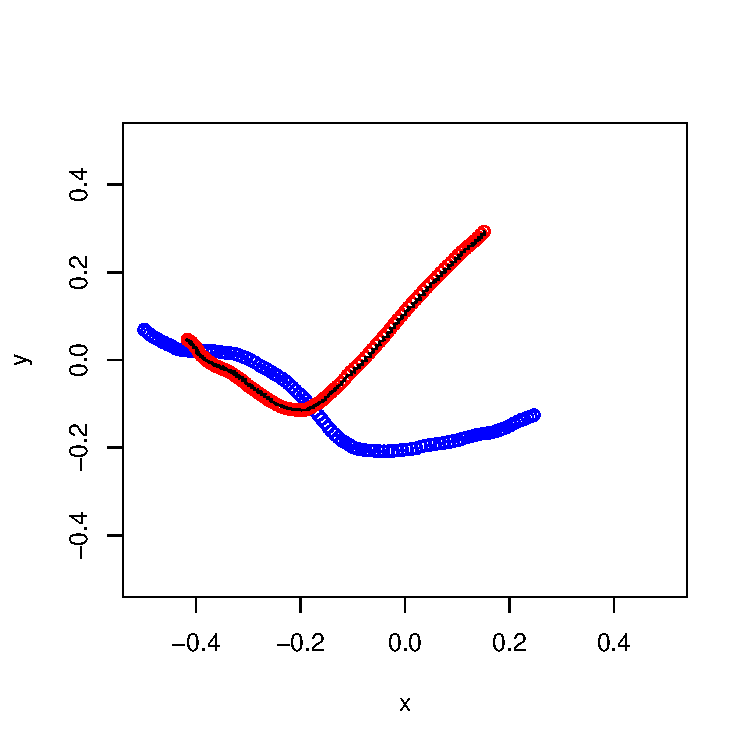
\includegraphics[width=3.25in]{nbaspatial}
\end{center}
\vspace{-0.25in}
\caption{The agreement between the black curve (mean of simulated
  stochastic pursuit trajectories using MAP estimated parameters) and
  the red curve (chaser's trajectory) shows that the stochastic
  pursuit model is appropriate.  The runner's trajectory is given in blue.}
\label{fig:nbaspatial}
\end{figure}

To visualize the insight provided by the model, we plot in Figure
\ref{fig:inferredgamma} the MAP
estimated $\gamma(t)$ function over the time period of the fast break,
$0 \leq t \leq 4.12$.  The speed $\gamma(t)$ is the piecewise constant
function plotted in black, while the mean speed computed directly from
the data is given by a red horizontal line.  The inferred speed shows
that the chaser slows down dramatically approximately $1.5$ seconds
into the fast break.  If one reviews the video footage of the play,
this corresponds to the runner confusing the chaser and evading him.

Given our stochastic pursuit model's success in fitting the real data,
in future work, we seek to apply the same methodology to a much larger
sample of fast breaks.  In this way, we can quantify a runner's
ability to evade a chaser and/or a chaser's ability to stay near a
runner who is actively trying to score.

\begin{figure}
\vspace{-0.5in}
\begin{center}
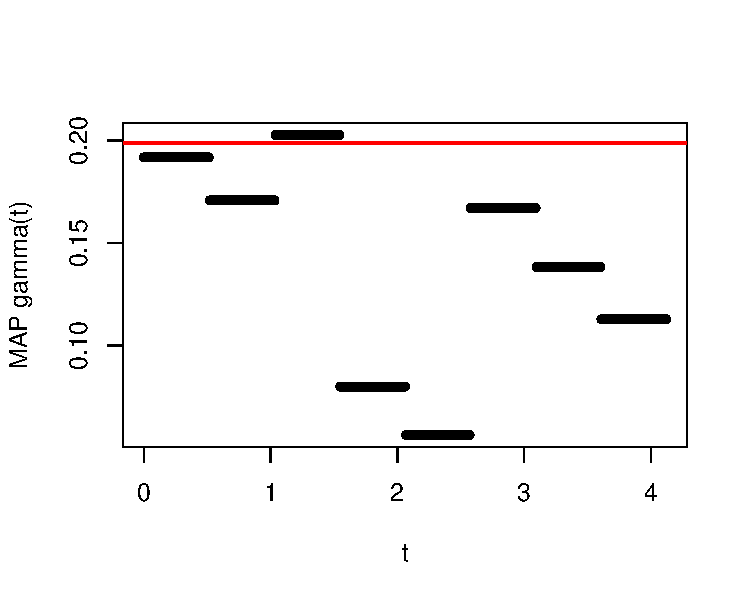
\includegraphics[width=3.25in]{inferredgamma}
\end{center}
\vspace{-0.25in}
\caption{For the fast break tracking data described in the text, we
  plot the MAP estimate of the chaser's speed $\gamma(t)$ in black.
  Note that the inferred speed differs greatly from the mean speed
  across the entire trajectory, plotted as a horizontal red line.}
\label{fig:inferredgamma}
\end{figure}

% \begin{acknowledgement}
% We gratefully acknowledge support from UC Merced's Committee on Research.
% \end{acknowledgement}

\vspace{-0.25in}

\bibliographystyle{spmpsci}
\bibliography{HMS2016}

\end{document}

%$$
%p^{n+1}(\mathbf{x};\theta) = \int_{y_1=x_1-\Gamma}^{y_1=x_1+\Gamma} \int_{y_2=x_2-\Gamma}^{y_2=x_2+\Gamma} K(x_1,x_2,y_1,y_2; \theta) p^n(\mathbf{x};\theta).
%$$

% To infer the unknown parameters $L, C, \sigma_1,$ and $\sigma_2$ in (\ref{eqn:sdeapplication}) we use simulated data of $X_{1,t}$, and $X_{1,t}$ as our observations. To simulate observations we use Euler-Maryama  sampling method after fixing the unknown parameters to some known values. For $1 \leq m \leq M$, let us approximate $t_m$ by $t_m \approx (n_m) h$ where $n_m = \lfloor t_m / h \rfloor$, an integer.  We make this approximation because, while we do want to allow the data to be taken at irregular times---perhaps with large gaps---we want to apply the Euler-Maruyama approximation on a fine, equispaced grid.


